\chapter{Large Language Model: Practice} \label{ch:llmpractice}

This chapter studies the selection, deployment and use of LLMs in production environment for different tasks.

\section{Python Environment Setup}

LLM provides APIs to interact with many different programming languages or platforms such as Python, JavaScript, and many more. In the scope of this chapter, we focus on Python-based LLM interaction, as Python is one of the most widely used language for ANN and LLM studies and applications development.

It is recommended to collect all the necessary libraries in a file, such as \texttt{environment.yml}, and use
\begin{lstlisting}
conda env create -f environment.yml --name <environment name>
\end{lstlisting}
to create an environment and install the packages all together. Anaconda shall figure out the dependencies and compatibility of the packages, and have everything installed correctly.

An example of such YAML file is given below. This example is taken from \cite{eddonner2025llm}.
\begin{lstlisting}
channels:
  - conda-forge
  - defaults
dependencies:
  - python=3.11
  - pip
  - python-dotenv
  - requests
  - numpy
  - pandas
  - scipy
  - pytorch
  - jupyterlab
  - ipywidgets
  - matplotlib
  - scikit-learn
  - chromadb
  - jupyter-dash
  - sentencepiece
  - pyarrow
  - faiss-cpu
  - pip:
    - beautifulsoup4
    - plotly
    - bitsandbytes
    - transformers
    - sentence-transformers
    - datasets
    - accelerate
    - openai
    - anthropic
    - google-generativeai
    - gradio
    - gensim
    - modal
    - ollama
    - psutil
    - setuptools
    - speedtest-cli
    - langchain
    - langchain-core
    - langchain-text-splitters
    - langchain-openai
    - langchain-chroma
    - langchain-community
    - faiss-cpu
    - feedparser
    - twilio
    - pydub
\end{lstlisting}

Among the libraries shown above, some are commonly used across all Python and machine learning projects such as \verb|numpy|, \verb|pandas| and \verb|scikit-learn|, while others are LLM specific packages such as \verb|transformer|, \verb|ollama| and \verb|langchain|.


\begin{shortbox}
\Boxhead{Environment Solutions of Anaconda Versus PyPA}

Anaconda is a Python distribution developed and maintained by Anaconda Inc. It provides \verb|conda|, a useful tool, to manage packages and environments. Anaconda provides reliable services to professional data scientists, cooperations as well as the free-of-charge services to the community. Python also has its native packages and environments management tools known as \verb|pip| and \verb|venv| developed and maintained by \myabb{Python Packaging Authority}{PyPA}.

Both \verb|conda| and \verb|pip| allow users to create an environment and install packages from a file. The commands are
\begin{lstlisting}
conda env create -f <filename> --name <environment name>
\end{lstlisting}
and
\begin{lstlisting}
python -m venv <environment name>
pip install -r <filename>
\end{lstlisting}
respectively.

It is of the user's choice whether to use \verb|conda| (from Anaconda, or its light version, Miniconda) or \verb|pip|/\verb|venv| to manage the packages. Under the scope of this notebook, both of them should fulfill the needs. As of this writing, the trend seems to be that data scientists, researchers and lectures would more often use \verb|conda|, while software engineers, \verb|pip|/\verb|venv|.
\end{shortbox}

\section{LLM Local Deployment}

Ollama and Langflow are introduced. Ollama allows fast deployment of an open-source LLM on a local computer, while Langflow is a low-code tool that allows a developer to easily integrate and test an LLM in a data pipeline.

\subsection{Quick LLM Deployment with Ollama}

Nowadays it is convenient to quickly deploy an open-source LLM on a PC with necessary hardware. One of the simplest way of doing that is to leverage on \mync{Ollama}, an open-source tool that allows the deployment of commonly seen open-source LLMs such as LLaMA, DeepSeek, etc., on a local machine. Notice that the usable LLMs are limited by the hardware power of the machine. During the installation of Ollama, it automatically detects and configures the GPU of the machine accordingly.

Once Ollama is installed, use
\begin{lstlisting}
ollama run <model name>
\end{lstlisting}
in the terminal to download and start a model. A screenshot is given in Fig. \ref{fig:ollama_llama32} as an example that runs LLaMA 3.2 with Ollama on a PC using the above command.

\begin{figure}[!htb]
	\centering
	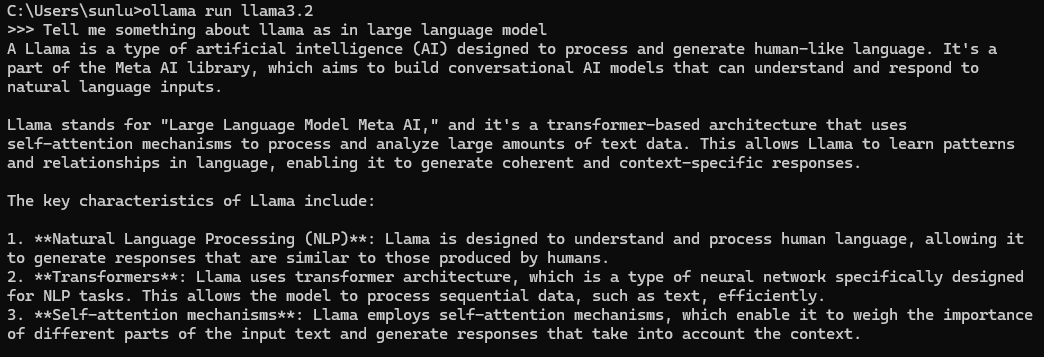
\includegraphics[width=\textwidth]{./chapters/part-7/figures/ollama_llama32.png}
	\caption{An example of running Ollama with LLaMA 3.2.}
	\label{fig:ollama_llama32}
\end{figure}

The deployed LLM does not come with any fancy graphical interface, but instead with the basic CLI. The user has the freedom to further deploy interfaces for applications on top of the basic interface. 

A list of Ollama supported LLMs are given in \cite{ollama2025library}. As of this writing, famous ones include \verb|deepseek-r1| (1.5B to 671B), \verb|llama3.3| (70B), \verb|llama3.2| (1B, 3B), \verb|gemma3| (1B to 27B), and a lot more. 

\subsection{Interaction with Locally Deployed LLM}

In the previous section, we learned that Ollama can be used to conveniently deploy an open-source LLM on the local machine, and it also provides a CLI where the user can chat with the LLM. It is possible to connect a Python program to that LLM using the interface that Ollama provides.

Make sure that the model is running in the backend. Start the model and check the model status using \verb|ollma serve| and \verb|ollama ps| respectively.

Python program can connect to the model either via HTTP request to \verb|http://localhost:11434/api/chat| as follows.
\begin{lstlisting}
import requests

OLLAMA_API = "http://localhost:11434/api/chat"
HEADERS = {"Content-Type": "application/json"}
MODEL = "llama3.2"

messages = [
    {"role": "user", "content": "<content of the message>"}
]
payload = {
        "model": MODEL,
        "messages": messages,
        "stream": False
    }
response = requests.post(OLLAMA_API, json=payload, headers=HEADERS)
print(response.json()['message']['content'])
\end{lstlisting}

Alternatively, use \verb|ollama| package as follows.
\begin{lstlisting}
import ollama

MODEL = "llama3.2"
messages = [
    {"role": "user", "content": "<content of the message>"}
]
response = ollama.chat(model=MODEL, messages=messages)
print(response['message']['content'])
\end{lstlisting}

OpenAI's Python package also provides tools to connect to local LLMs like what has been deployed via Ollama.

\begin{lstlisting}
from openai import OpenAI

MODEL = "llama3.2"
messages = [
    {"role": "user", "content": "<content of the message>"}
]
ollama_via_openai = OpenAI(base_url='http://localhost:11434/v1', api_key='ollama')
response = ollama_via_openai.chat.completions.create(
    model=MODEL,
    messages=messages
)
print(response.choices[0].message.content)
\end{lstlisting}

\subsection{Naive Deployment}

Ollama uses C++ to compile an LLM and deploy it on the local machine. The compiled model is easy to use and runs efficiently, but it is generally difficult to modify—such as for fine-tuning or architectural changes.

For users seeking more flexibility, it is possible to download the raw parameters of open-source LLMs and run them independently. Many such models are available from platforms like Hugging Face, allowing users to experiment with customization, fine-tuning, or integration into custom pipelines. But of course, there will be additional steps for the users to execute the models, and they are introduced in this section.




\section{LLM Cloud Deployment}

Many companies provide the user with cloud-based LLMs. These LLMs are often more powerful and robust than locally deployed ones. 

\subsection{Browser-Based Chatbot}

Companies such as OpenAI, Google, Microsoft and Deepseek provide web-based chatbot interface where a user can directly chat with the model. Many of these companies also provide APIs that allow user program to connect to models running on the cloud.

\subsection{Cloud-Service-Provider-Managed LLM Deployment}

Nowadays many cloud providers including AWS, Microsoft Azure, Google Cloud Service, etc., that allow the user to deploy LLM models on their servers. For example, AWS provides Amazon Bedrock which is its frontier model that can be easily deployed on AWS. Similar applies to other major cloud service providers.

\subsection{API-Based LLM}

Many LLM service providers, such as OpenAI, allows the user to interact with their cloud-based LLMs using APIs through command lines. Notice that the API-based LLM has a completely different business model compared with the chatbot, and should be treated as different services.

If the user has decided to use a commercialized LLM model via its API key, he needs to register an account with the LLM provider, such as OpenAI, and create a new API key, and added it to the project as an environmental variable. 

Notice that the use of the API key often introduces costs to be paid to the LLM provider. The cost depends on the model and the number of input and output tokens in a call. To give a perspective, as of this writing the cost of OpenAI's API calls are given in Table \ref{tab:openai_api_price} as of this writing. Powerful models such as \texttt{o1} are significantly more expansive than less powerful ones such as \texttt{gpt-4o-mini}. This is different from chatbot service where the user pays a fixed monthly subscription fee and get almost unlimited access to most of the models of his choice.

\begin{table}
	\centering \caption{OpenAI's API Calls Pricing as of this writing, in USD per $1M$ tokens.}\label{tab:openai_api_price}
	\begin{tabular}{lrr}
		\hline
		Model & Input Cost & Output Cost \\ \hline
        \texttt{gpt-5} & $1.25$ & $10.00$ \\
        \texttt{gpt-5-mini} & $0.25$ & $2.00$ \\
        \texttt{gpt-5-nano} & $0.05$ & $0.40$ \\
        \texttt{gpt-4.1} & $2.00$ & $8.00$ \\
        \texttt{gpt-4.1-mini} & $0.40$ & $1.60$ \\
        \texttt{gpt-4.1-nano} & $0.10$ & $0.40$ \\
        \texttt{gpt-4o} & $2.50$ & $10.00$ \\
        \texttt{gpt-4o-mini} & $0.15$ & $0.60$ \\
        \texttt{o1} & $15.00$ & $60.00$ \\
        \texttt{o1-pro} & $150.00$ & $600.00$ \\
		\hline
	\end{tabular}
\end{table}

The details about the registration of the account and the creation of the API key are not included in this notebook.

The Python library \verb|openai| provides a quick way to interact with its models, given that the user has a valid API key. A basic realization looks like the following. An example is given later. The ``completions'' API is used, which asks the LLM to complete a conversation.
\begin{lstlisting}
from openai import OpenAI

api_key = '<sk-proj-...>' # put api key here

openai = OpenAI(api_key=api_key)
messages = [
{"role": "system", "content": "<system prompt>"},
{"role": "user", "content": "<user prompt>"}
]
response = openai.chat.completions.create(model="<model>", messages=messages)
\end{lstlisting}

The format of \verb|message|, originally defined by OpenAI, has now become a convention for LLM API calls. In the message, \verb|<system prompt>| tells LLM the basic setup, such as what role the LLM shall play and what it should do, whereas \verb|user prompt| gives the user specific data that the LLM needs to process.

An example connecting to \verb|gpt-4o-mini| is given below.

\begin{lstlisting}
import os
from openai import OpenAI
from dotenv import load_dotenv

load_dotenv(override=True) # api key is loaded as an environment variable

openai = OpenAI()
message = "Hello, GPT! I am connecting you via your API. Let's see how it works."
response = openai.chat.completions.create(model="gpt-4o-mini", messages=[{"role":"user", "content":message}])
print(response.choices[0].message.content)
\end{lstlisting}

For the above code to work, make sure that \verb|.env| file exists, and environment variable \verb|OPENAI_API_KEY| has been setup inside.

A response similar to the following can be obtained.
\begin{lstlisting}
Hello! It's great to hear that you're connecting via the API. How can I assist you today?
\end{lstlisting}

A typical \verb|messages| that is passed to OpenAI often looks like the following
\begin{lstlisting}
messages = [
    {"role": "system", "content": "<system prompt>"},
    {"role": "user", "content": "<user prompt>"},
    {"role": "assistant", "content": "<LLM historical response>"},
    {"role": "user", "content": "<user prompt>"},
    {"role": "assistant", "content": "<LLM historical response>"},
    {"role": "user", "content": "<user prompt>"}
]
\end{lstlisting}
where \verb|<system prompt>| tells LLM the basic setup, such as what role the LLM shall play and what it should do, whereas \verb|<user prompt>| gives the user specific data that the LLM needs to process. LLM API by itself is stateless. The historical conversations need to be passed to it to retain a long conversation. In that case, \verb|assistant| role is used to store LLM's historical responses, so that it knows which part comes from the user and which part from the historical itself.

OpenAI and other companies such as Google, Deepseek, etc., provide variety of APIs for different functions. More details are introduced in later sections.

\subsection{Commonly Seen APIs}

OpenAI GPT, Anthropic Claude and Google Gemini are used as examples. Their supported commonly used APIs are introduced below, with examples to demonstrate the syntax. 

\section{Model Fine-Tuning}

Many LLM service providers such as OpenAI allows a user to fine-tune a clone of their base models using his own data. The user pays the computation resources consumed during the fine tuning, and the fine-tuned model needs to reside at the servers of the service provider. Alternatively, a user can also download open-source models from the community, such as Hugging Face, and fine-tune a model locally.

This section introduces the practices in model fine-tuning. To start, a brief review of some of the frontier models is given as of this writing.

\subsection{A Review of Frontier Models} \label{sec:frontierllmmodels}

Models to be reviewed in this section are summarized in Table \ref{tab:frontiermodels}. It is also indicated in the table whether the model is propriety or open-source, whether the corresponding company provides a browser-based chatbot where the user can quickly test its performance, and whether the corresponding company provides API call services where the user can link an application to the LLM running at the company's servers.

\begin{table}[!htb]
	\centering
	\caption{Frontier LLMs and their accessibility features.} 
	\label{tab:frontiermodels}
	\begin{tabular}{lccc}
		\hline
		Model (Company) & Proprietary / Open-Source\textsuperscript{1} & Chatbot\textsuperscript{2} & API\textsuperscript{3} \\
		\hline
		GPT (OpenAI)           & P & Y & Y \\
		Claude (Anthropic)     & P & Y & Y \\
		Gemini (Google)        & P & Y & Y \\
		LLaMA (Meta)           & O & N & N \\
		Qwen (Alibaba)         & O & Y & Y \\
		DeepSeek (DeepSeek)    & O & Y & Y \\
		\hline
	\end{tabular}
	
	\vspace{0.5em}
	\begin{flushleft}
		\tiny
		Note: A model may have multiple versions or variants with different accessibility features. This table reflects the latest version of each model line as of this writing. \\
		\textsuperscript{1} Proprietary / Open-Source: Whether the model weights are publicly released and can be deployed locally. \\
		\textsuperscript{2} Chatbot: Whether an official website hosted by the developer allows users to interact with the model. Costs may apply, even for open-source models. \\
		\textsuperscript{3} API: Whether the developer provides official API access. Costs may apply, even for open-source models.
	\end{flushleft}
\end{table}


OpenAI's GPT model is probably the earliest and most well known LLM among the general public. It was also one of the first models to support multimodal inputs. Today, many third-party applications developed by independent developers default to using GPT when integrating an LLM. The latest version, GPT-4o, is highly capable and performs well across a wide range of general tasks.

Claude is well regarded among data scientists and is considered one of the most powerful LLMs on the market. Claude models are famous for their capability in mathematics, programming and logic reasoning.

Gemini is Google’s flagship LLM family, designed to integrate tightly with its broader ecosystem. The latest versions of Gemini support multimodal inputs—including text, images, audio, and video—and are positioned to compete at the frontier of model capabilities.

Meta’s LLaMA series is one of the most influential open-source LLM families. It is commonly used as a foundation for fine-tuned or quantized models in local deployments. Many research institutions, particularly those not training models from scratch, choose LLaMA as their base, making it one of the most popular models in academia.

Qwen is Alibaba’s open-source LLM series, notable for its strong multilingual support and solid performance in both base and chat variants. It has achieved top rankings on several Chinese language benchmarks. As of this writing, Alibaba has released multiple specialized versions of Qwen for different downstream tasks.

DeepSeek models are open-source and gaining traction in both research and developer communities due to their strong performance and ease of access. Released under the permissive MIT license, DeepSeek stands out for its efficient architectural design and training strategy, enabling it to compete with top-tier models at a relatively low computational cost.





\subsection{Proprietary Model Fine-Tuning}

\subsection{Open-Source Model Fine-Tuning}

\section{Resource Augmented Generator}
